% \input{/Users/jovo/Research/latex/latex_paper.tex}

\documentclass[10pt,journal,cspaper,compsoc]{IEEEtran}
%
% If IEEEtran.cls has not been installed into the LaTeX system files,
% manually specify the path to it like:
% \documentclass[12pt,journal,compsoc]{../sty/IEEEtran}

\usepackage{fixltx2e}
% \usepackage{stfloats}
\usepackage{amsmath}
\usepackage{graphicx}
\usepackage{amsfonts}
\usepackage{amsthm}
\usepackage{cite}
\usepackage{algorithm}
\usepackage{algorithmic}
\usepackage{url}
\usepackage{enumerate}
% \usepackage{hyperref}
% 


\newcommand{\jv}{Joshua Vogelstein}
\newcommand{\jhu}{Johns Hopkins University}
%\newcommand{\hp}{https://jshare.johnshopkins.edu/jvogels3/public_html/}
\newcommand{\ema}{joshuav@jhu.edu}

\newcommand{\Vr}{V_{reset}}
\newcommand{\Vl}{V_{leat}}
\newcommand{\eqdef}{\overset{\triangle}{=}}
% \newcommand{\D}[2]{\frac{\partial #1}{\partial #2}}
\newcommand{\DD}[2]{\frac{\partial ^2 #1}{\partial #2 ^2}}
\newcommand{\DDD}[3]{\frac{\partial ^2 #1}{\partial #2 \partial #3}}
\newcommand{\Di}[2]{\frac{\partial ^i #1}{\partial #2 ^i}}
\newcommand{\grad}{\nabla}
\newcommand{\Hess}{\nabla\nabla}

\providecommand{\tg}[1]{\textcolor{green}{#1}}
\providecommand{\tb}[1]{\textcolor{blue}{#1}}
\providecommand{\tr}[1]{\textcolor{red}{#1}}
\providecommand{\tk}[1]{\textcolor{black}{#1}}
\providecommand{\twhite}[1]{\textcolor{white}{#1}}
\providecommand{\ve}[1]{\boldsymbol{#1}}
\providecommand{\ma}[1]{\boldsymbol{#1}}
%\providecommand{\ve}[1]{\boldsymbol{#1}}
%\newcommand{\norm}[1]{\left|\left|#1\right|\right|}
\providecommand{\norm}[1]{\left \lVert#1 \right  \rVert}
\providecommand{\deter}[1]{\lvert #1 \rvert}
\providecommand{\abs}[1]{\left \lvert #1 \right \rvert}
\providecommand{\mat}[1]{\left[ #1 \right]}
\newcommand{\trans}[1]{{#1}^{\ensuremath{\mathsf{T}}}}           % transpose
\newcommand{\transpose}[1]{{#1}^{\ensuremath{\mathsf{T}}}}           % transpose
\newcommand{\argmax}{\operatornamewithlimits{argmax}}
\newcommand{\argmin}{\operatornamewithlimits{argmin}}
\newcommand{\T}{^{\ensuremath{\mathsf{T}}}}           % transpose

\newcommand{\XX}{\mathbb{X}}         
\newcommand{\CC}{\mathbb{C}}         
\newcommand{\FF}{\mathbb{F}}         
\newcommand{\PP}{\mathbb{P}}         
\newcommand{\GG}{\mathbb{G}}         
\newcommand{\EE}{\mathbb{E}}           % expected value
\newcommand{\II}{\mathbb{I}}           % indicator function
\newcommand{\QQ}{\mathbb{Q}}           
\newcommand{\SSS}{\mathbb{S}}           
\newcommand{\YY}{\mathbb{Y}}
\newcommand{\Aa}{\mathbb{A}}
\newcommand{\VV}{\mathbb{V}}
\newcommand{\LL}{\mathbb{L}}
\newcommand{\ZZ}{\mathbb{Z}}         

\newcommand{\iid}{\overset{iid}{\sim}}

% \DeclareMathOperator*{\argmax}{argmax}
% \DeclareMathOperator*{\argmin}{argmin}
% \DeclareMathOperator{\find}{find}

% \newtheorem{thm}{Theorem}
\newcommand{\thma}{\begin{thm}}
\newcommand{\thmb}{\end{thm}}

\newcommand{\mata}{\begin{bmatrix}}
\newcommand{\matb}{\end{bmatrix}}



\newtheorem{lemma}{Lemma}
\newtheorem{Rem}{Remark}%[section]
\newtheorem{Alg}{Algorithm}%[section]
\newtheorem{thm}{Theorem}
\newtheorem{Thm}{Theorem}[section]
\newtheorem{Lem}{Lemma}[section]
\newtheorem{defi}{Definition}
\newtheorem{Def}{Definition}[section]
\newtheorem{prop}{Proposition}
\newtheorem{coro}[thm]{Corollary}
\newtheorem{claim}{Claim}
\newtheorem{conj}{Conjecture}
% \newtheorem{corollary}{Corollary}
% \newtheorem{theorem}{Theorem}
%\theoremstyle{marginbreak}
%\newtheorem{Lem}[Cor]{Lemma}
%\theoremstyle{change}
%\theorembodyfont{\itshape}


% \newtheorem{defi}{Definition}
% \newcommand{\defa}{\begin{defi}}
% \newcommand{\defb}{\end{defi}}

% \newcommand{\eq}{\begin{equation}}
% \newcommand{\en}{\end{equation}}
% \newcommand{\eqa}{\begin{equation}}
% \newcommand{\eqb}{\end{equation}}

\newcommand{\enuma}{\begin{enumerate}}
\newcommand{\enumb}{\end{enumerate}}
\newcommand{\ena}{\begin{enumerate}}
\newcommand{\enb}{\end{enumerate}}

\newcommand{\itema}{\begin{itemize}}
\newcommand{\itemb}{\end{itemize}}
\newcommand{\ita}{\begin{itemize}}
\newcommand{\itb}{\end{itemize}}

\newcommand{\proofa}{\begin{proof}}
\newcommand{\proofb}{\end{proof}}

\newcommand{\bla}{\begin{block}}
\newcommand{\blb}{\end{block}}

% \newcommand{\seqa}{\begin{equation*}}
\newcommand{\seqb}{\end{equation*}}

\newcommand{\bth}{\ve{\theta}}
\newcommand{\hth}{\mh{\theta}}
\newcommand{\htth}{\mh{\theta}}
\newcommand{\bhth}{\mh{\ve{\theta}}}
\newcommand{\thetn}{\ve{\theta}}
\newcommand{\thet}{\thetn}
\newcommand{\theth}{\widehat{\ve{\theta}}}
\newcommand{\theto}{\ve{\theta}'}
\newcommand{\wht}{\widehat{\thet}}
\newcommand{\wtt}{\widetilde{\thet}}
\newcommand{\vth}{\ve{\thet}}
\newcommand{\vTh}{\ve{\Theta}}
\newcommand{\hvth}{\widehat{\ve{\thet}}}
\newcommand{\bTh}{\ve{\Theta}}
\newcommand{\hbth}{\widehat{\thet}}

% \newcommand{\p}{P_{\bth}}
\newcommand{\pold}{P_{\bth'}}
\newcommand{\pk}{P_{\widehat{\ve{\theta}}^{(k)}}}
\newcommand{\pT}{P_{\thetn_{Tr}}} %\thetn_T
\newcommand{\pO}{P_{\thetn_o}} %\thetn_o
% \newcommand{\Q}{Q(\thetn,\theto)}
% \newcommand{\m}{m^{\ast}}
% \newcommand{\q}{q(\ve{H}_t)}
\newcommand{\Ca}{[\text{Ca}^{2+}]}

\newcommand{\Lik}{\mathcal{L}}
\newcommand{\Cae}{[\widehat{\text{Ca}}^{2+}]}
\newcommand{\Cav}{\ve{C}}%[\ve{\text{Ca}}^{2+}]}
\newcommand{\sml}{\sqrt{\ma{\lambda}}}
\newcommand{\ml}{\ma{\lambda}}
\newcommand{\nw}{\widehat{n}}
\newcommand{\nv}{\vec{n}}
\newcommand{\Ae}{\widehat{A}}
\newcommand{\te}{\widehat{\tau}}
\newcommand{\maxn}{\max_{\ve{n}: n_t \geq 0}}
% \newcommand{\V}{\text{Var}}

\providecommand{\mc}[1]{\mathcal{#1}}
\providecommand{\mb}[1]{\boldsymbol{#1}}
\providecommand{\mbb}[1]{\mathbb{#1}}
\providecommand{\mv}[1]{\vec{#1}}
\providecommand{\mh}[1]{\hat{#1}}
\providecommand{\mt}[1]{\widetilde{#1}}
\providecommand{\mhc}[1]{\hat{\mathcal{#1}}}
\providecommand{\mtc}[1]{\widetilde{\mathcal{#1}}}
\providecommand{\mhb}[1]{\hat{\boldsymbol{#1}}}
\providecommand{\mvb}[1]{\vec{\boldsymbol{#1}}}
\providecommand{\mtb}[1]{\widetilde{\boldsymbol{#1}}}

\newcommand{\mP}{\mathbb{P}}

\newcommand{\del}{\delta}
\newcommand{\sig}{\sigma}
\newcommand{\lam}{\lambda}
\newcommand{\gam}{\gamma}
\newcommand{\eps}{\varepsilon}

\newcommand{\Del}{\Delta}
\newcommand{\Sig}{\Sigma}
\newcommand{\Lam}{\Lambda}
\newcommand{\Gam}{\Gamma}

\newcommand{\dvs}{\dot{\bs}_t}
\newcommand{\dvw}{\dot{\bw}_t}
\newcommand{\dvx}{\dot{\bx}_t}
\newcommand{\dvy}{\dot{\by}_t}

\newcommand{\ft}{f_{\ve{\thet}}}
\newcommand{\gt}{g_{\ve{\thet}}}
\newcommand{\hht}{h_{\thetn}}

\newcommand{\Real}{\mathbb{R}}

\newcommand{\wconv}{\overset{i.p.}{\rightarrow}}
\newcommand{\sconv}{\overset{i.p.}{\rightarrow}}
\newcommand{\conv}{\rightarrow}
\newcommand{\pconv}{\overset{p}{\conv}}
\newcommand{\mcE}{\mathcal{E}}
\newcommand{\mcT}{\mathcal{T}}
\newcommand{\mcG}{\mathcal{G}}
\newcommand{\mcM}{\mathcal{M}}
\newcommand{\mcL}{\mathcal{L}}
\newcommand{\hatmcE}{\widehat{\mcE}}
\newcommand{\hatp}{\widehat{p}}
\newcommand{\hatP}{\widehat{P}}
\newcommand{\hatQ}{\widehat{Q}}
\newcommand{\hatL}{\widehat{L}}
\newcommand{\mhP}{\widehat{\PP}}
\newcommand{\tildeA}{\widetilde{A}}

\newcommand{\defa}{\begin{defi}}
\newcommand{\defb}{\end{defi}}
\newcommand{\defeq}{\overset{\triangle}{=}}

\newcommand{\rqap}{\texttt{rQAP} }
\newcommand{\rqapa}{\texttt{rQAP}$_1$ }
\newcommand{\rqapb}{\texttt{rQAP$_{100}$} }
\newcommand{\rqapm}{\texttt{rQAP$_m$} }


% \renewcommand{\algorithmicrequire}{\textbf{Input:}}
% \renewcommand{\algorithmicensure}{\textbf{Output:}}



% \newcommand{\ss}{\mc{S}}
% \newcommand{\mhc}{\mh{\mc{S}}_n}

% \newcommand{\Real}{\mathbb{R}}
% \newcommand{\bTh}{\mb{\Theta}}
% \newcommand{\ra}{\rightarrow}
% \newcommand{\la}{\leftarrow}
% \newcommand{\bx}{\mb{x}}
% \newcommand{\bv}{\mb{v}}
% \newcommand{\ba}{\mb{a}}
% \newcommand{\bd}{\mb{d}}
% \newcommand{\balpha}{\mb{\alpha}}
% \newcommand{\conv}{\rightarrow}  
% \newcommand{\xx}{\langle \bx_u^\la, \bx_v^\ra\rangle}  
% \DeclareMathOperator*{\argmax}{arg \hspace{1pt} max \hspace{2pt}}
% \DeclareMathOperator*{\argmin}{arg \hspace{1pt} min \hspace{2pt}}
% \newcommand{\norm}[1]{\left \lVert#1 \right  \rVert}
% 


\newcommand{\theHalgorithm}{\arabic{algorithm}}


\DeclareMathOperator{\Delti}{\mathbf{\Delta}^{-1}}
\DeclareMathOperator{\Delt}{Q} %\mathbf{\Delta}}
% \DeclareMathOperator{\Gam}{\mathbf{\Gamma}}
\DeclareMathOperator{\Gami}{\mathbf{\Gamma}^{-1}}
\DeclareMathOperator{\Sigb}{\mathbf{\Sigma}}
\DeclareMathOperator{\Ri}{\mathbf{\R}^{-1}}
\DeclareMathOperator{\A}{A}
\DeclareMathOperator{\W}{\mathbf{W}}
\DeclareMathOperator{\V}{\mathbf{V}}
\DeclareMathOperator{\U}{\mathbf{U}}
\DeclareMathOperator{\C}{\mathbf{C}}
\DeclareMathOperator{\uvec}{\mathbf{u}}
\DeclareMathOperator{\D}{\mathbf{D}}
\DeclareMathOperator{\Q}{\mathbf{Q}}
\DeclareMathOperator{\R}{R} %\mathbf{P}}
\DeclareMathOperator{\Y}{\mathbf{Y}}
\DeclareMathOperator{\B}{\mathbf{B}}
\DeclareMathOperator{\Hmat}{\mathbf{H}}
\DeclareMathOperator{\Gmat}{\mathbf{G}}
\DeclareMathOperator{\X}{\mathbf{X}}
\DeclareMathOperator{\Cmat}{C} %\mathbf{L}}
\DeclareMathOperator{\Pmat}{\mathbf{P}}
\DeclareMathOperator{\veta}{\mathbf{\mb{v}}}
\DeclareMathOperator*{\minimize}{\mathrm{minimize}}
\DeclareMathOperator*{\maximize}{\mathrm{maximize}}
\DeclareMathOperator*{\Ymod}{\mathbf{\Y}}
\DeclareMathOperator*{\Bmod}{\mathbf{B}}
\DeclareMathOperator*{\Hmod}{\mathbf{H}}
\DeclareMathOperator*{\Lmod}{\mathbf{L}}
\DeclareMathOperator*{\Xmod}{\mathbf{\X}}
% \DeclareMathOperator*{\mb{v}mod}{\mathbf{\mb{v}}}





\hyphenation{op-tical net-works semi-conduc-tor}
% \newcommand{\Qqap}{\Qqap}
\usepackage{caption}
\captionsetup{justification=raggedright}
\newcommand{\PmcP}{P \in \mc{P}}


\begin{document}

\title{Fast Inexact Graph Matching \\ with Applications in Statistical Connectomics}
% \title{A Quadratic Assignment Problem Approach to Graph Matching: Applications in Statistical Connectomics}

\author{Joshua T.~Vogelstein, John M.~Conroy, Louis J.~Podrazik, Steven G.~Kratzer, 
        Donniell E.~Fishkind, 
		R.~Jacob~Vogelstein,
        and~Carey~E.~Priebe% <-this % stops a space
\IEEEcompsocitemizethanks{\IEEEcompsocthanksitem J.T. Vogelstein, D.E. Fishkind, and C.E. Priebe are with the Department
of Applied Mathematics and Statistics, Johns Hopkins University, Baltimore, MD 21218. 
%\protect\\
% note need leading \protect in front of \\ to get a newline within \thanks as
% \\ is fragile and will error, could use \hfil\break instead.
E-mail: \{joshuav,def,cep\}@jhu.edu, \{conroyjohnm,ljpodra,sgkratz\}@gmail.com, jacob.vogelstein@jhuapl.edu
\IEEEcompsocthanksitem J.M. Conroy, L.J. Podrazik and S.G. Kratzer are with Institute for Defense Analyses, Center for Computing Sciences, Bowie, MD 20708.
\IEEEcompsocthanksitem R.J. Vogelstein is with the Johns Hopkins University Applied Physics Laboratory, Laurel, MD, 20723.}% <-this % stops a space
\thanks{This work was partially supported by the Research Program in Applied Neuroscience.}}
 
% The paper headers
\markboth{UNDER REVIEW}%
{Graph Classification}

\IEEEcompsoctitleabstractindextext{%
\begin{abstract}
	It is becoming increasingly popular to represent myriad and diverse data sets as graphs.  When the labels of vertices of these graphs are unavailable, graph matching (GM)---the process of determining which permutation assigns vertices of one graph to those of another---is a computationally daunting problem.  This work presents an inexact strategy for GM.  Specifically, we frame GM as a quadratic assignment problem, and then relax the feasible region to its convex hull.  We prove that our relaxed optimization function has the same solution as the original problem, yet it is continuously differentiable. Because the objective function is not necessarily convex, we consider multiple principled initializations.  Performance exceeds the previous state-of-the-art in \emph{all} of 16 benchmark tests.  Moreover, this approach is fast, scaling cubically with the number of vertices, requiring only about a minute on a laptop for graphs with a few hundred vertices.  We illustrate this approach via a brain-graph application (the Caenorhabditis elegans ``connectome'').  We find that we can find the optimal solution for nearly every random permutation of the connectome that we sample.  Although this strategy already natively operates on weighted graphs, either directed or undirected, we propose a number of possible extensions, and make all code available.
\end{abstract}

% Note that keywords are not normally used for peer review papers.
\begin{keywords}
statistical inference, graph theory, network theory, structural pattern recognition, connectome.
\end{keywords}}


% make the title area
\maketitle
\IEEEdisplaynotcompsoctitleabstractindextext
\IEEEpeerreviewmaketitle



\section{Introduction}

% define a graph labeling function as any algorithm that assigns a label to each vertex of a graph: $Q_n: \mc{A}, \Xi^n \mapsto \mc{L}$, where $\Xi \subseteq \mc{G}$, for example, $\Xi=\mc{A}$ (note that we have actually defined a sequence of graph labeling functions).  Remember that we have defined $\mc{L}$ as a subset of $[n_v]$, so each vertex need not have a unique label.  

\IEEEPARstart{A}{} graph matching (GM) algorithm is any algorithm whose goal is to ``align'' any pair of graphs such that each vertex in one graph can be ``assigned'' to its corresponding vertex in the other graph.  Perhaps due to its complex computational properties (it is $\mc{NP}$-hard \cite{Garey1979}), GM has received widespread attention in both the mathematical graph theory and computer science communities \cite{Conte2004}.  Moreover, the potential span of applications of graph matching algorithms is vast, ranging from neural coding \cite{Richiardi2010} to machine vision \cite{Wiskott1997}.  

Our motivation for this work includes the bourgeoning field called ``connectomics'': the study of brain-graphs.  In brain-graphs,  vertices represent (collections of) neurons and edges represent either functional dependencies or structural connections \cite{Sporns2010}.  In some scenarios, vertices are labeled.  For example, when vertices represent single neurons in invertebrates \cite{WhiteBrenner86} or macro-anatomical gyral regions in vertebrates \cite{Biswal2010,Bullmore2010}.  However, in other scenarios, even whether vertices can be labeled is questionable.  For example, if one desired to compare brain-(sub)graphs from parts of brains across species or within vertebrate organisms, there is no known vertex assignment.  In these scenarios GM might be an important element of any statistical analysis of these brain-graphs \cite{VP11_sigsub, VP11_unlabeled}.


We therefore propose a novel inexact graph matching algorithm based on the quadratic assignment problem (QAP).  The intuition is relatively simple: GM is computationally difficult because the underlying feasible region is non-differentiable and the implied objective function is multimodal.  A common approach to approximating difficult nonlinear programming problems is to relax the constraints on the feasible region.  By relaxing the non-differentiable constraint, any gradient based algorithm may be applied to the problem \cite{Mangasarian1987}. Importantly, our relaxed version of the optimization problem (rQAP) yields an identical solution to the original QAP problem whenever the two graphs are simple and isomorphic. Unfortunately, the multimodality of the solution space implies that the initialization will, in general, be important.  Multiple ``principled'' restarts can potentially facilitate an efficient stochastic search strategy.  

This manuscript describes an algorithm that approximately solves a relaxed version of graph matching in cubic time (with very small leading constants).  Via numerical experiments, we demonstrate that this approach outperforms several state-of-the-art algorithms on all tests in a standard benchmark library \cite{Burkard1997}, indicating both its efficiency and its effectivity. We then test this approach on a brain-graph matching problem: matching the brain-graph (connectome) of a small nematode with $302$ vertices with a permuted version of itself.  We are able to find the optimal solution after $3$ restarts for each randomly permuted example of its chemical connectome, and typically $<30$ restarts for each randomly permuted example of its electrical connectome.  We are therefore optimistic that this algorithm will be useful for the massive graphs ($\mc{O}(10^5)$ vertices)  promised to arise due to various ongoing connectome projects \cite{HCP,OCP}.










% \section{Methods} % (fold)
% \label{sec:methods}


\section{Graph  Matching} % (fold)
\label{sub:preliminaries}

% subsection preliminaries (end)

A labeled graph $G=(\mc{V},\mc{E})$ consists of a vertex set $\mc{V}$, where $|\mc{V}|=n$ is number of vertices and an edge set $\mc{E}$, where $|\mc{E}| \leq n^2$. Note that we are not restricting our formulation to be directed or exclude self-loops. Given a pair of graphs, $G_1=(\mc{V}_1,\mc{E}_1)$ and $G_2=(\mc{V}_1,\mc{E}_1)$, where $|\mc{V}_1|=|\mc{V}_2|=n$, 
let $\pi: \mc{V}_1 \to \mc{V}_2$ be a permutation function (bijection),
and let $\Pi$ be the set of all such permutation functions.  Now consider the following two closely related problems:
% A pair of graphs, $G_1$ and $G_2$, are isomorphic if and only if the following \emph{isomorphism criterion} holds: there exists a $\pi \in \Pi$ such that . 
% Let $A$ be the adjacency matrix representation of graph such that $A_{uv}=1$ if there is an edge from $u$ to $v$, and $A_{uv}=0$ otherwise. 
% Note that the below follows for directed/undirected and loopy/non-loopy graphs.
% $u \sim v \in \mc{E}$ and $A_{uv}=0$ otherwise.  
% Let  $\Pi$ be the set of permutation functions, where a permutation function (bijection) $\pi: \mc{V} \to \mc{V}$ (re-)orders the elements of the set $\mc{V}$.  Given a pair of $n \times n$ adjacency matrices, $A=(a_{uv})$ and $B=(b_{uv})$, consider the following two problems:
\begin{itemize}
	\item \textbf{Graph Isomorphism (GI):}  Does there exist a $\pi \in \Pi$ such that $(u,v) \in \mc{E}_1$ if and only if $(\pi(u),\pi(v)) \in \mc{E}_2$. 
		\item \textbf{Graph Matching (GM):} Which $\pi$ (if any) satisfies the above isomorphism criterion?
\end{itemize}

% \begin{itemize}
% 	% $\PmcP$ (if any) satisfies $QAQ\T=B$?
% 	\item \textbf{Linear Assignment Problem (LAP):} 
% 	\begin{align}
% 		\text{minimize}_{\pi \in \Pi} \sum_{u \in \mc{V}} a_{u \pi(v)}
% 	\end{align}
% 	\item \textbf{Quadratic Assignment Problem (QAP):} 
% 	\begin{align}
% 		\text{minimize}_{\pi \in \Pi} \sum_{u,v \in \mc{V}} a_{\pi(u) \pi(v)}b_{uv}
% 	\end{align}
% \end{itemize}

Both GI and GM are computationally difficult. GM is at least as hard as GI, since solving GM also solves GI, but not vice versa. It is not known whether GI is in complexity class $\mc{P}$ \cite{Fortin1996}.  In fact, GI is one of the few problems for which, if $\mc{P} \neq \mc{NP}$, then GI might reside in an intermediate complexity class called $\mc{GI}$-complete.  GM, however, is known to be $\mc{NP}$-hard.    
 % There exist no known algorithms for which worst case behavior is polynomial \cite{Fortin1996}.  While GM is known to be $\mc{NP}$-hard, it remains unclear whether GI is in $\mc{P}$, $\mc{NP}$, or its own intermediate complexity class, $\mc{NP}$-isomorphism (or isomorphism-complete).  
Yet, for large classes of GI and GM problems, linear or polynomial time algorithms are available \cite{Babai1980}.  Moreover, at worst, it is clear that GI is only ``moderately exponential,'' for example, $\mc{O}(\exp\{n^{1/2 + o(1)}\})$ \cite{Babai1981}.  Unfortunately, even when linear or polynomial time GI or GM algorithms are available for special cases of graphs, the constants are typically unbearably large.  For example, if all graphs have degree less than $k$, there is a linear time algorithm for GI.  However, the hidden constant in this algorithm is $512k^3!$ \cite{Chen1994}.  

Because we are interested in solving GM for graphs with $\mc{O}(10^6)$ or more vertices, exact GM solutions will be computationally intractable. As such, we develop a fast inexact graph matching algorithm.   Our approach is based on formulating GM as a quadratic assignment problem.  Below, we introduce assignment problems, and reiterate their close relationship to GI and GM \cite{Burkard2009}.

% We therefore determined the average complexity of our algorithm \emph{and} the leading constants.  Figure \ref{fig:scaling} suggests that our algorithm is not just cubic in time, but also has very small leading constants ($\approx 10^{-7}$ seconds), making using this algorithm feasible for even reasonably large graphs.


\section{Assignment Problems} % (fold)
\label{sub:assignment_problems}

Both GI and GM can be cast as assignment problems.  Let $A=(a_{uv})$ and $B=(b_{uv})$ correspond to the adjacency matrix representations of graphs $G_1$ and $G_2$, respectively.  That is, $a_{uv}=1$ if and only if $(u,v) \in \mc{E}_1$, and zero otherwise (and similarly for $B$ and $G_2$). Now, GI may be stated thusly:  does there exist a $\pi \in \Pi$ such that $a_{uv}=b_{\pi(u)\pi(v)}$ for all $u,v \in [n]=\{1,\ldots, n\}$.  Although assignment problems do not restrict $A$ and $B$ to correspond to adjacency matrices, when $A$ and $B$ are adjacency matrices, GM and the quadratic assignment problem (QAP) are equivalent.  Our approach is based on a continuous relaxation and quadratic optimization approach, as will be described below.  Because a linear assignment problem (LAP) will be a subroutine of our approach, we introduce LAP first, followed by QAP.   A permutation matrix is a matrix $P=(p_{uv})$ that satisfies the following three conditions:
\begin{enumerate}
\item	$P\mb{1} = \mb{1}$,
\item	$P\T \mb{1}=\mb{1}$, %\\
\item 	$P \in  \{0,1\}^{n \times n}$.	
\end{enumerate}
Let $\mc{P}$ be the set of all such permutation matrices. Note that while the first two constraints are linear, the third constraint is \emph{binary}.  This nonlinearity motivates our approach.
	 %\\
% \end{align}




% Given a pair of adjacency matrices, $A$ and $B$, to graph match $A$ with $B$ is to find a permutation matrix $Q$ such that $QAQ\T=B$. In this work, we propose a novel inexact graph matching algorithm, essentially a Frank-Wolfe algorithm with multiple restarts.  We demonstrate the efficacy of this algorithm over the previous state-of-the-art on a reference library of benchmarks.  


\subsection{Linear Assignment Problems} % (fold)
\label{ssub:linear_assignment_problems}

% subsubsection linear_assignment_problems (end)

The standard way of writing LAP is
\begin{subequations} \label{eq:LAP}
\begin{align}
	 \text{(LAP) }\quad  &\underset{\pi}{\text{minimize}} \sum_{u,v \in [n]} a_{u \pi(v)} b_{uv} \\
	&\text{subject to } \pi \in \Pi,
\end{align}
\end{subequations}
which can be written equivalently in a number of ways using the notion of permutation matrix introduced above:
\begin{subequations} \label{eq:LAP2}
\begin{align}
	&\argmin_{\PmcP} \norm{PA - B}_F =\\
	&\argmin_{\PmcP} \, tr(PA-B)\T (PA-B)=\\ 
	% &\argmin_{\PmcP} tr (A\T P\T PA) - tr(2PAB\T) + tr(B\T B)=\\ 
	&\argmin_{\PmcP}  -tr (P AB\T) = \argmin_{\PmcP}  -\langle P\T, AB\T \rangle = \label{eq:2c} \\
	% &\argmin_{\PmcP}  -\sum_{u,v \in [n]} p_{uv} a_{uv} b_{vu}
	% =\\% &\argmin_{\PmcP}  - \text{vec}(P)\T \text{vec}(AB\T).=\\
	&\argmin_{\PmcP}  -\langle P, AB\T \rangle, \label{eq:dotLAP}
\end{align}
\end{subequations}
where $\langle \cdot,\cdot \rangle$ %the equality on the second to last line defines 
is the usual Euclidean inner product, i.e., $\langle X,Y\rangle := tr(X\T,Y)= \sum_{ij} x_{ij} y_{ij}$.  
While the objective function and the first two constraints of LAP are linear, the binary constraints make solving this problem computationally tricky.  Nonetheless, in the last several decades, there has been much progress in accelerating algorithms for solving LAPs, starting with exponential time, all the way down to $\mc{O}(n^3)$ for general LAPs, and even faster for certain special cases (e.g., sparse matrices) \cite{Jonker1987, Burkard2009}.
% The last form indicates that LAP is a linear programming problem (hence the name).  Yet, the constraints, $\mc{P}$, make it a bit trickier.  The feasible region $\mc{P}$ can be written as a set of three constraints: two linear equality constraint sets and a binary constraint.  The LAP objection function with constraints can explicitly be written:
% \begin{align}
% 		&\text{minimize}_P  &&\sum_{u \in \mc{V}} -p_{uv} a_{uv} b_{vu} \nonumber \\
% 		&\text{subject to } && \sum_{u \in \mc{V}} p_{uv} = 1 \, \forall u \in \mc{V} \nonumber \\
% 		& && \sum_{v \in \mc{V}} p_{uv} = 1 \, \forall v \in \mc{V}, \nonumber \\
% 		& &&p_{uv} \in \{0,1\} \, \forall u,v. \label{eq:rLAP}	
% \end{align}
% Perhaps because LAP comes up in a wide variety of contexts, a large number of algorithms have been developed to solve LAP \cite{Burkard2009}.  These algorithms have become increasing efficient.  
% One of the most popular algorithms, the so-called ``Hungarian algorithm'' has time complexity $\mc{O}(n^3)$ \cite{Jonker1987}.  Under certain conditions (for example, when $AB\T$ is sparse), faster implementations are also available.  As will be seen below, LAP is a key subroutine to our inexact QAP solution.  

Consider a continuous relaxation of LAP.  
A matrix $P$ is doubly stochastic precisely when $P$ satisfies the following three conditions: 
\begin{enumerate}
\item	$P\mb{1} = \mb{1}$,
\item	$P\T \mb{1}=\mb{1}$, %\\
\item 	$P \in  \Real_+^{n \times n}$,
\end{enumerate}
where the third constraint relaxes the binary constraints of the permutation matrices with a non-negativity constraint.  
Let $\mc{D}$ be the set of doubly stochastic matrices.
With this, we now state a relaxed LAP problem:
\begin{subequations} \label{eq:rLAP}
\begin{align}
		\text{(rLAP) } \quad &\underset{P}{\text{minimize}}  &&-\langle P, AB\T \rangle \\
		&\text{subject to } && P \in \mc{D}.
		% && \sum_{u \in \mc{V}} p_{uv} = 1 \, \forall u \in \mc{V} \nonumber \\
		% 		& && \sum_{v \in \mc{V}} p_{uv} = 1 \, \forall v \in \mc{V}, \nonumber \\
		% 		& &&p_{uv} \geq 0 \, \forall u,v, \label{eq:ALAP}	
\end{align}
\end{subequations}
As it turns out, solving rLAP is equivalent to solving LAP.
\begin{prop}
	LAP and rLAP are equivalent, meaning that they have the same optimal objective function value.
\end{prop}
\begin{proof}
	Although this proposition is typically proven by invoking total unimodularity, we present a simpler proof here.	Let $P'$ be a solution to LAP and let $P = \sum_{i\in[k]} \alpha_i P^{(i)}$ be a solution to rLAP for some positive integer $k$, permutation matrices $\{P^{(i)}\}_{i \in [k]}$, and positive real numbers $\{\alpha_i\}_{i \in[k]}$ such that $\sum_{i \in [k]} \alpha_i=1$.  Note that 
	\begin{align*}
	\langle P,AB\T \rangle &= \langle  \sum_{i\in[k]} \alpha_i P^{(i)}, AB\T \rangle=  \sum_{i\in[k]} \alpha_i \langle  P^{(i)}, AB\T \rangle	 \\
	&\leq \sum_{i\in[k]} \alpha_i \langle P', AB\T  \rangle = \langle P', AB\T \rangle \leq \langle P, AB\T \rangle,
	\end{align*}
	% then we have a contradiction, 
	because $P'$ is feasible in rLAP.
	\end{proof}
This relaxation motivates our approach to approximating QAP.

	
 
% Originally formulated in the BLAH-BLAH form, LAP has received much attention in the last several decades \cite{???}. While the original solutions required $\mc{O}(n^6)$ time, recent implementations of the ``Hungarian algorithm'' require only $\mc{O}(n^3)$ or less \cite{???}.\footnote{More efficient algorithms are available for certain special cases, for example, whenever the matrix-vector multiplication operation is fast (for example, when both $A$ and $B$ are sparse).} As will be evident in a subsequent section, solving a LAP will be the primary computational bottleneck in our approach.   

\subsection{Quadratic Assignment Problems} % (fold)
\label{ssub:linear_assignment_problems}

% subsubsection linear_assignment_problems (end)

Koopmans and Beckman \cite{Koopmans1957} introduced QAP in its original form:
\begin{subequations}
\begin{align}
	\text{(QAP) } \quad &\underset{\pi}{\text{minimize}}  &&\sum_{u,v \in [n]} a_{\pi(u)\pi(v)} b_{uv}  \\
	&\text{subject to } && \pi \in \Pi.
\end{align}
\end{subequations}
More recently, a number of equivalent formulations have been developed:
\begin{subequations} \label{eq:QAP}
\begin{align}
	&\argmin_{\PmcP} \norm{PAP\T - B}_F = \\
	 % &\argmin_{\pi \in \Pi} \sum_{u \in \mc{V}} A_{\pi(u) \pi(v)} B_{uv} =\\
	% &\argmin_{\PmcP} \norm{PAP\T - B}_F =
	% \\&
	% \argmin_{\PmcP} \norm{PA - BP\T} =\\
	% &\argmin_{\PmcP} (PAP\T-B)\T (PAP\T-B) \\ 
	&\argmin_{\PmcP} tr(PAP\T - B)\T (PAP\T - B)  = \\
	% &\argmin_{\PmcP}  tr(P\T A\T P\T P A P\T) - 2tr(PAP\T B) + tr(B\T B)  = \\ %- tr(B\T PAP\T)
	&\argmin_{\PmcP} - tr(B\T PAP\T)= \label{eq:trQAP}\\ % - tr(PAP\T B),			
	% &\argmin_{\PmcP} tr (A\T P\T PA) - tr(2PA) + tr(B\T B)=\\ 
	% &\argmin_{\PmcP}  - tr(B\T PAP\T)=\\
	% &\argmin_{\PmcP}  -\sum_{u \in \mc{V}} p_{uv} a_{uv} b_{uv} p_{vu} 
	% = \\ &\argmin_{\PmcP}  -\langle PAP\T, B \rangle.
	% 
	&\argmin_{\PmcP}  -\langle B,PAP\T \rangle.
	 % =\\
\end{align}
\end{subequations}
Our approach follows from relaxing the binary constraint from the trace formulation of the problem, Eq. \eqref{eq:trQAP}.  Specifically, we desire to solve the following relaxed QAP problem:
\begin{subequations} \label{eq:rQAP}
\begin{align}
		\text{(rQAP) } \quad &\underset{P}{\text{minimize}}  && - tr(B\T PAP\T)  \\
		&\text{subject to } && P \in \mc{D}.
\end{align}
\end{subequations}
rQAP is therefore a quadratic problem with linear constraints, meaning that relatively standard solvers may be employed.


Importantly, the convex hull of permutation matrices is the set of doubly stochastic matrices, implying that this is a ``natural'' relaxation in a very meaningful sense.    Moreover, although the objective function $- tr(B\T PAP\T)$ is quadratic, it is not necessarily convex.  This follows from computing the Hessian of the objective function with respect to $P$:
\begin{align}
	\nabla_P^2  =  B \otimes A + B\T \otimes A\T,
\end{align}
which is not necessarily positive definite ($\otimes$ indicates the Kronecker product). This means that the solution space will potentially be multimodal, making initialization important.  With this in mind, below, we describe an algorithm to find a local optimum of rQAP.


\section{Fast Inexact Graph Matching Algorithm} % (fold)
\label{ssub:graph_matching}


Our strategy has three components:
\begin{enumerate}[I.]
	\item Choose an initial estimate.
	\item Find a local solution to Eq. \eqref{eq:rQAP}.
	\item Project that solution onto the set of permutation matrices.
\end{enumerate}
We refer to one run of the above three steps as \texttt{rQAP}.  For any integer $m$, upon using $m$ restarts, we report only the best solution, and we refer to the whole procedure as \texttt{rQAP}$_m$.  Below, we provide details for each component.

\textbf{I: Find a suitable initial position $P^{(0)} \in \mc{D}$}  While any doubly stochastic matrix would be a feasible initial point, two choices seem natural: (i) the ``flat doubly  stochastic matrix,'' $J=\ve{1} \cdot \ve{1}\T/n$, which is the center of the feasible region, and (ii) the identity matrix, which is a permutation matrix.  Therefore, if we run \rqap  once, we always start with one of those two.  If we use multiple restarts, each initial point is ``near'' the flat matrix.  Specifically, we sample $K$, a random doubly stochastic matrix using 10 iterations of Sinkhorn balancing \cite{Sinkhorn1964}, and let $P^{(0)}=(J+K)/2$. %Given this initial estimate, we iterate the following five steps until convergence.


\textbf{II: Find a local solution to Eq. \eqref{eq:rQAP}} As mentioned above, Eq. \eqref{eq:rQAP} is a quadratic problem with linear equality and boundary constraints.  A number of off-the-shelf algorithms are readily available for finding local optima in such problems.  We utilize the Frank-Wolfe (FW) algorithm, which is both (i) a kind of projection descent algorithm
% called the 
% We therefore develop a nonlinear programing algorithm for approximately solving Eq. \eqref{eq:rQAP} using multiple restarts.
   % Our approach can be thought of as a 
% Frank-Wolfe (FW) algorithm, which is also 
and (ii) a successive linear programming algorithm.  The FW algorithm was originally designed for solving quadratic problems with linear (equality and/or inequality) constraints \cite{Frank1956}. It later became used more generally for nonlinear programming problems  \cite{Bradley1977}.  Specifically, it can be used to solve optimization problems of the following form:
\begin{subequations} \label{eq:FW}
\begin{align}
		\text{(FWP) } \quad &\underset{x}{\text{minimize}}  && f(x)  \\
		&\text{subject to } && x \in \mc{S},
\end{align}
\end{subequations}
where $\mc{S} \subset \Real^d$ is a polyhedral set (a set described by linear constraints) and the function $f: \mc{S} \to \Real$ is continuously differentiable.  Generally, the Frank-Wolfe algorithm consists of the following steps.  Given an initial position, $x^{(0)}$, recurse the following steps until some convergence criterium (e.g., computational budget) is met.  Let $\mt{x}^{(i)}$ be the optimal solution that minimizes the first order Taylor series approximation of $f$ around $x^{(i)}$ such that  $\mt{x}^{(i)} \in \mc{S}$.  Next, let $x^{(i+1)}$ minimize $f(x)$ such that $x^{(i+1)}$ is on the line segment from $x^{(i)}$ to $\mt{x}^{(i)}$ in $\mc{S}$.  
% The function $\mt{f}^{(i)}: \mc{S} \to \Real$ is defined to be the first-order (i.e., linear) approximation to $f$ at $x^{(i)}$---that is $f^{(i)} := f(x^{(i)}) + \nabla f(x^{(i)})\T (x-x^{(i)})$.  Next, solve the following linear program: minimize $\mt{f}^{(i)}(x)$ such that $x \in \mc{S}$ (this can be done efficiently since it is a linear objective function with linear constraints).  Note that by ignoring additive constants the objective function of this subproblem can be abbreviated: minimize $\nabla f(x^{(i)})\T x$ such that $x \in \mc{S}$.  Let $\mt{x}^{(i)}$ be the solution to this problem.  Now, the point $x^{(i)} \in \mc{S}$ is defined as the solution to: minimize $f(x)$ such that $x$ is on the line segment from $x^{(i)}$ to $\mt{x}^{(i)}$ in $\mc{S}$.  Because this is a one-dimensional quadratic optimization problem, it can be analytically solved exactly.   Go to the next $i$ and terminate this iterative procedure when $x^{(i)}$ stops changing much or develops a gradient sufficiently close to zero.
% The FW algorithm iteratively finds the direction of steepest descent, projects the direction into the feasible region, and takes a step of optimal size.  

Below we provide a detailed view of applying FW to rQAP.  Given an initial position, $P^{(i)}$, iterate the following four steps.

\emph{Step 1: Compute the gradient $\nabla f(P^{(i)})$:}  The gradient $f$ with respect to $P$ is given by
% \emph{Step 1: Compute the gradient} The gradient of $f$ with respect to $P$ is given by
\begin{align} \label{eq:grad}
	\nabla f (P^{(i)}) = 
	% \partial f / \partial P^{(i)} =
	  - A P^{(i)} B\T - A\T P^{(i)} B.
\end{align}


\emph{Step 2: Compute the direction $\mt{P}^{(i+1)}$:} The direction is giving by that which minimizes a first order Taylor series approximation to $f(P)$ around the current estimate, $P^{(0)}$: The first order Taylor series approximation to $f(P)$ is given by
\begin{align}
	\mt{f}^{(i)}(P) := f(P^{(i)}) + \nabla f(P^{(i)})\T(P - P^{(i)})
\end{align}
Thus, Step 1 of FW is
% \begin{align}
% 		\text{(FW1) } \quad &\underset{P}{\text{minimize}}  && \mt{f}(P)  \\
% 		&\text{subject to } && P \in \mc{D},
% \end{align}
% which is equivalent to
\begin{subequations} \label{eq:FW1}
\begin{align}
	\mt{P}^{(i+1)} = \argmin_{P \in \mc{D}} &f(P^{(i)}) + \nabla f(P^{(i)})\T(P - P^{(i)}) 
	=\\ \argmin_{P \in \mc{D}} &\nabla f(P^{(i)})\T P 
	= \\ \argmin_{P \in \mc{D}} & \langle \nabla f(P^{(i)}), P \rangle, \label{eq:dotFW1}
\end{align}
\end{subequations}
which is a LAP.  This can be seen by considering Eq. \eqref{eq:dotLAP}.  Let $A=\nabla_P^{(i)}$ and $B=I$ (the $n\times n$ identity matrix), and Eq. \eqref{eq:dotFW1} is identical to Eq. \eqref{eq:dotLAP}.

% Thus, we can solve the first step of FW upon computing 

\emph{Step 3: Compute the step size $\alpha^{(i)}$} Given $\mt{P}^{(i+1)}$, the new direction is given maximizing the \emph{original} optimization problem, Eq. \eqref{eq:rQAP}, along the line segment from $P^{(i)}$ to $\mt{P}^{(i+1)}$ in $\mc{D}$.    
% 
% \begin{align}
% 	d^{(i)}=L^{(i)}-P^{(i)}.
% \end{align}
% 
% % paragraph step_3_updating_the_direction (end)
% 
% \emph{Step 4: Line search} Given this direction, one can then perform a line search to find the doubly stochastic matrix that minimizes the objective function along that direction:
\begin{align}\label{eq:step}
	\alpha^{(i)} = \argmin_{\alpha \in [0,1]} f(P^{(i)} + \alpha^{(i)} \mt{P}^{(i)}).
\end{align}
This can be performed exactly, because $f$ is a quadratic function.  

% paragraph step_4_line_search (end)

\emph{Step 4: Update $P^{(i)}$} Finally, the new estimated doubly stochastic matrix is given by
\begin{align}\label{eq:update}
	P^{(i+1)} = P^{(i)} + \alpha^{(i)} \mt{P}^{(i+1)}.
\end{align}

% paragraph step_5_update_q_ (end)

\emph{Stopping criteria} Steps 1--4 are iterated until some stopping criterion is met (computational budget limits, $P^{(i)}$ stops changing much, or $\nabla f(P^{(i)})$ is close to zero).  These four steps collectively comprise the FW algorithm for solving Eq. \eqref{eq:rQAP}.  %Note that while $P^{(i)}$ will generally not be a permutation matrix, we do not project $P^{(i)}$ back onto the set of permutation matrices between each iteration, as that projection requires $\mc{O}(n^3)$ time.


\textbf{III: Projecting onto the set of permutation matrices}   Let $P^{(I)}$ be the doubly stochastic matrix resulting from the final iteration.  We project $P^{(I)}$ onto the set of permutation matrices, yielding
\begin{align} \label{eq:proj}
	\mh{P} = \argmin_{\PmcP} -\langle P^{(I)}, P \rangle,
\end{align}
which is a LAP.  Thus, this completes one restart of \texttt{rQAP}.

% paragraph the_final_iteration (end)

% \textbf{Multiple restarts} We refer to multiple re-starts of \rqap with subscripts; that is, the performance of \rqapm is the best result of $m$ pseudo-random re-starts of \texttt{rQAP}.  We continue restarting until either we converge to a known global solution or we exceed our computational budget. Note that \rqap natively operates on matrices, which could correspond to either weighted or unweighted, directed or undirected graphs.  

% Algorithm \ref{alg:1} shows pseudo-code for the complete algorithm.

% 
% \begin{algorithm}
% 	\begin{algorithmic}[1]
% 		\REQUIRE $A$, $B$, $n_{max}$, convergence criteria
% 		\ENSURE $\mh{Q}$
% 		\FOR{$n=1,\ldots, n_{max}$}
% 		\STATE Initialize estimate $Q^{(0)}$
% 		\FOR{$j=1,2,\ldots$}
% 		\STATE Do \rqap until convergence
% 		% \STATE Find closest doubly stochastic matrix using Eq. \eqref{eq:LAP} using the Hungarian algorithm
% 		% \STATE Update the direction using Eq. \eqref{eq:dir}
% 		% \STATE Find optimal step size using Eq. \eqref{eq:step}
% 		% \STATE Obtain new estimate using Eq. \eqref{eq:update}
% 		% \IF{converged} break \ELSE continue 
% 		% \ENDIF  
% 		\ENDFOR
% 		\ENDFOR
% 	\end{algorithmic}
% \end{algorithm}

% paragraph putting_it_all_together (end)
% subsubsection graph_matching (end)


\section{Theoretical Results} % (fold)
\label{sec:theoretical_results}

\subsection{LAP vs. QAP} % (fold)
\label{sub:lap_vs_qap}

At surface, LAP and QAP are quite similar.  In fact, the gradient of the LAP objective function is $2AB\T$.
% Much like the QAP objective function from Eq. \eqref{eq:QAP} can be simplified to Eq. \eqref{eq:QAP}, the LAP objective function can be similarly simplified, to give
% \begin{align}
% 	Q_{LAP}= \argmin_{\PmcP} \norm{QA-B}_F^2 = \argmin_{\PmcP} tr(QA B\T).
% \end{align}
% The gradient of the argument on the right-hand-side of the above equation is $2AB\T$.
% Letting $f_{LAP}(Q)=tr(QA B\T)$, the gradient is:
% \begin{align}
% 	% f_{QAP}(Q)	&= -tr(B\T QAQ\T) -tr(QAQ\T B)  &f_{LAP}(Q)&=-tr(AQ\T B\T) \\
% 	% \nabla_{QAP}&= AQB\T+A\T QB               	&
% 	\nabla_{LAP}&=2A B\T.
% \end{align}
% Thus, when $Q=I$, the gradient of the QAP objective function is identical to that of the LAP objective function. Thus, one can use gradient ascent to to solve a LAP.  The gradient of $f'(Q)=\norm{AQ\T-B}_F^2$ is %:
% % \begin{align} \label{eq:grad2}
% 	$\partial f'/\partial Q = 2A B\T$. 
% % \end{align}
Comparing this gradient to the gradient of the QAP objective function---Eq. \eqref{eq:grad}---one can see that when (i) $P^{(i)}$ is the identity matrix and (ii) both $A$ and $B$ are symmetric (for example, for undirected graphs), the two gradients are identical.  Thus, if QAP is initialized at the identity matrix and the graphs are undirected, the first permutation matrix---the output of \emph{Step 2} in our \rqap algorithm---is identical to the LAP solution; although the line search will make $P^{(1)}$ not equal the LAP solution in general. %$ \neq Q_{LAP}$, in general.  %Moreoever, projecting a matrix onto the closest permutation matrix can be written as a LAP because of the following relationship:
% \begin{align}
% 	\argmin_{\PmcP} \norm{QA\T - I}_F^2 &= \argmin_{\PmcP} (QA\T-I)\T (QA\T-I) 
% \nonumber\\ &=\argmin_{\PmcP} AQ\T QA\T -2QA\T - II = \argmin_{\PmcP}  -\langle Q, A\T \rangle  
% \end{align}

% In the above simulation, the first iteration of \rqap is essentially the only useful one.  Thus, we compare the performance of \texttt{BPI}$\circ$\texttt{LAP} (dark gray).  The performance of LAP and QAP are not statistically different for this simulation.  This suggests that for certain problems, LAP (which is $\mc{O}(n^3)$) is both an efficient and useful approximation to solving $\mc{NP}$-hard graph matching problems. We were unable to find a model for simple graphs in which multiple iterations of \rqap improved performance over LAP. %We confirm this intuition by substituting QAP with LAP in the above simulations (black line).  As depicted in the above figures, this intuition is consistent with the numerical results. In other words, while naively one might implement an algorithm with exponential time complexity, LAP, which is only quadratic time complexity, will often suffice.


% subsection lap_vs_qap (end)

\subsection{rQAP solves QAP in certain special cases} % (fold)
\label{sub:rqap_solves_qap_}

Although, rLAP and LAP are always equivalent, in general, it is not the case that rQAP and QAP are equivalent.  However, in a certain important special case, rQAP and QAP are equivalent.
\begin{thm}
	If $A$ and $B$ are the adjacency matrices of simple graphs (symmetric, hollow, and binary) that are isomorphic to one another, then the minimum of rQAP is equal to the minimum QAP.
\end{thm}
\begin{proof}
Because any feasible solution to QAP is also a feasible solution to rQAP, we must only show that the optimal solution to rQAP can be no better than the optimal solution to QAP.  Let $A=PBP\T$, so that $\langle A, PBP\T\rangle=2m$, where $m$ is the number of edges in $A$.  If rQAP could achieve a lower objective value, then it must be that there exists a $D \in \mc{D}$ such that $\langle A, DBD\T\rangle > \langle A, PBP\T\rangle = 2m$ (remember that we are minimizing the negative Euclidean inner product). For that to be the case, it must be that $(DBD\T)_{uv} \geq 1$ for some $(u,v)$.  That this is not so may be seen by the submultiplicativity of the $\ell_{\infty}$ norm:
$\norm{Px}_\infty \leq \norm{P}_\infty \norm{x}_\infty$.  Applying this twice (once for each permutation matrix multiplication) yields our result.
% Consider $d_i=\langle D, \text{col}_i(BD\T) \rangle$, where $\text{col}_i(\cdot)$ indicates the $i^{th}$ column of the matrix.  $d_i \leq 1$ for all $i \in [n]$, therefore, our result holds.
\end{proof}
% subsection rqap_solves_qap_ (end)


% section theoretical_results (end)

\section{Numerical Results} % (fold)
\label{sub:numerical_results}


% subsection numerical_results (end)

\subsection{QAP benchmarks}

To assess numerical properties or \texttt{rQAP}$_m$, we compare its performance with recent state-of-the-art approaches on the QAP benchmark library \cite{Burkard1997}.  Specifically, \cite{Zaslavskiy2009} reported improved performance in all but two cases, in which the QPB method of Cremers et al. \cite{Schellewald2001} achieved a lower minimum.  
% We compare \rqapm with the previous state-of-the-art algorithm.  
In \emph{all} cases, \texttt{rQAP}$_3$ outperforms the previous best result, often by orders of magnitude in terms of relative error. In three cases, \rqapb achieves the absolute minimum.  In 12 out of 16 cases, the simple \rqapa algorithm outperforms the others (starting with the flat doubly stochastic matrix).  See Figure \ref{fig:fwpath} for quantitative comparisons.


% \begin{table}[h!]
% \caption{Comparison of Frank-Wolfe with Minimum Solution and Previous State-of-the-Art (PSOA)}
% \begin{center}
% \begin{tabular}{|r|r|r||r|r|r|r|r|}
% \hline
% \# & Problem  &   Min    & \rqapb & \texttt{rQAP}$_{3}$ & \texttt{rQAP}$_{2}$ & \rqapa & PSOA\\
% \hline
% 1&    chr12c &   11156 &   12176 &   13072 &   13072 &   13072 &   18048\\
% 2&    chr15a &    9896 &    9896 &   17272 &   17272 &   27584 &   19086\\
% 3&    chr15c &    9504 &   10960 &   14274 &   14274 &   17324 &   16206\\
% 4&   chr20b &    2298 &    2786 &    3068 &    3068 &    3068 &    5560\\
% 5&    chr22b &    6194 &    7218 &    7876 &    7876 &    8482 &    8500\\
% 6&    esc16b &     292 &     292 &     294 &     294 &     320 &     296\\
% 7&     rou12 &  235528 &  235528 &  238134 &  253684 &  253684 &  256320\\
% 8&     rou15 &  354210 &  356654 &  371458 &  371458 &  371458 &  381016\\
% 9&     rou20 &  725522 &  730614 &  743884 &  743884 &  743884 &  778284\\
% 10&    tai10a &  135028 &  135828 &  148970 &  157954 &  157954 &  152534\\
% 11&    tai15a &  388214 &  391522 &  397376 &  397376 &  397376 &  419224\\
% 12&    tai17a &  491812 &  496598 &  511574 &  511574 &  529134 &  530978\\
% 13&    tai20a &  703482 &  711840 &  721540 &  721540 &  734276 &  753712\\
% 14&    tai30a & 1818146 & 1844636 & 1890738 & 1894640 & 1894640 & 1903872\\
% 15&    tai35a & 2422002 & 2454292 & 2460940 & 2460940 & 2460940 & 2555110\\
% 16&    tai40a & 3139370 & 3187738 & 3194826 & 3194826 & 3227612 & 3281830\\
%     \hline
% \end{tabular}
% \end{center}
% \label{tab:fwpath}
% \end{table}%

\begin{figure}[htbp]
	\centering			
	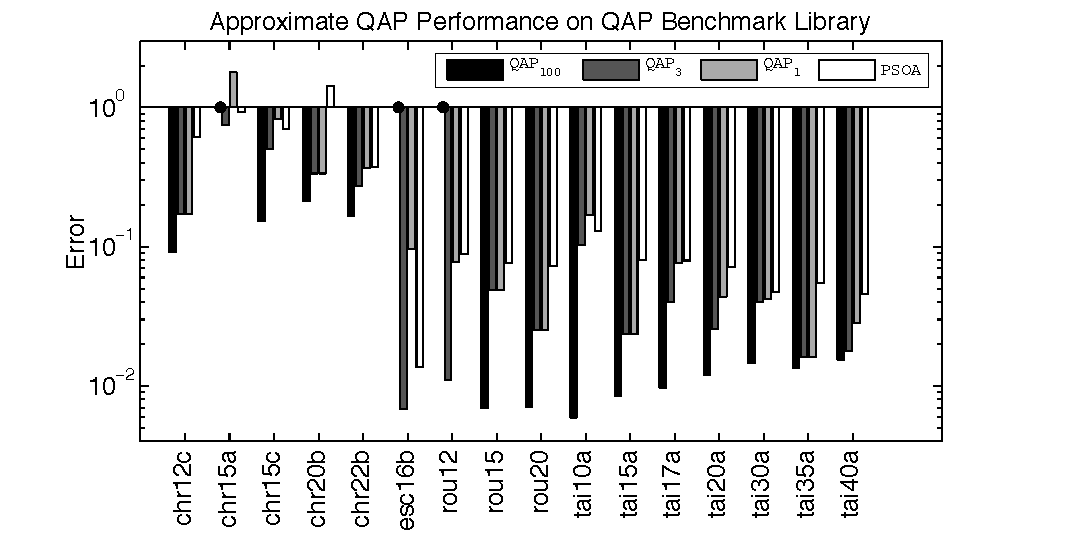
\includegraphics[width=1.0\linewidth]{benchmarks.pdf}
	\caption{\texttt{rQAP}$_3$ outperforms the previous state-of-the-art (PSOA) on all 16 benchmark graph matching problems.  Moreover, \rqapa outperforms PSOA on 12 of 16 tests.  For 3 of 16 tests, \rqapb achieves the minimum (none of the other algorithms ever find the absolute minimum), as indicated by a black dot.  Let $f_*$ be the minimum and $\mh{f}_x$ be the minimum achieved by algorithm $x$.  Error is $\mh{f}_x/f_*-1$.  }
	\label{fig:fwpath}
\end{figure}




\subsection{Algorithm Complexity and leading constants} % (fold)
\label{sub:algorithm_complexity_and_leading_constants}

% Both GM and its closely related counterpart, graph isomorphism (GI), are computationally difficult.  There exist no known algorithms for which worst case behavior is polynomial \cite{Fortin1996}.  While GM is known to be $\mc{NP}$-hard, it remains unclear whether GI is in $\mc{P}$, $\mc{NP}$, or its own intermediate complexity class, $\mc{NP}$-isomorphism (or isomorphism-complete).  Yet, for large classes of GI and GM problems, linear or polynomial time algorithms are available \cite{Babai1980}.  Moreover, at worst, it is clear that GI is only ``moderately exponential,'' for example, $\mc{O}(\exp\{n^{1/2 + o(1)}\})$ \cite{Babai1981}.  Unfortunately, even when linear or polynomial time GM or GI algorithms are available for special cases of graphs, the constants are typically unbearably large.  For example, if all graphs have degree less than $k$, there is a linear time algorithm for GI.  However, the hidden constant in this algorithm is $512k^3!$ \cite{Chen1994}.  
As mentioned above, GM is computationally difficult; even those special cases for which polynomial time algorithms are available, the leading constants are intractably large for all but the simplest cases. We therefore determined the average complexity of our algorithm \emph{and} the leading constants.  Figure \ref{fig:scaling} suggests that our algorithm is not just cubic in time, but also has very small leading constants ($\approx 10^{-7}$ seconds), making using this algorithm feasible for even reasonably large graphs.




\begin{figure}[htbp]
	\centering			
	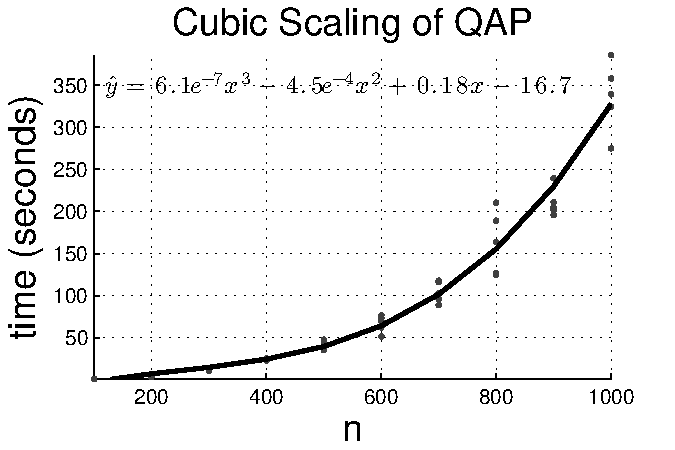
\includegraphics[width=1.0\linewidth]{digraph_qap2}
	\caption{Performance of \rqap as function of number of vertices. Data was sampled from an Erd\"os-R\'enyi model with $p=log(n)/n$.  Each dot represents a single simulation.  The solid line is the best fit cubic function.  Note the leading constant is $10^{-7}$ seconds. }
	\label{fig:scaling}
\end{figure}

% subsection algorithm_complexity_and_leading_constants (end)


\subsection{Brain-Graph Matching} % (fold)
\label{sub:connectome_classification}

A ``connectome'' is a brain-graph in which vertices correspond to (collections of) neurons, and edges correspond to connections between them. The \emph{Caenorhabditis elegans} (\emph{C. elegans}) is a small worm (nematode) with $302$ labeled vertices.  We consider the subgraph with $279$ somatic neurons that form edges with other neurons \cite{WhiteBrenner86, Varshney2011}.  Two distinct kinds of edges exist between vertices: chemical and electrical ``synapses'' (edges). Any pair of vertices may have several edges of each type. Moreover, some of the synapses are hyperedges amongst more than two vertices.    Thus, the connectome of a \emph{C. elegans} may be thought of as a weighted multi-hypergraph, where the weights are the number of edges of each type.  The \rqapm algorithm natively operates on weighted or unweighted graphs.  We therefore conducted the following synthetic experiments.  Let $A_{uvz} \in \{0,1,2,\ldots\}$ be the number of synapses from neuron $v$ to neuron $u$ of type $z$ (either chemical or electrical), and let $A_z=\{A_{uv}\}_{u,v \in [279]}$ for $z \in \{e,c\}$ corresponding to the electrical or chemical connectome.  Let $B_{iz}=Q_{iz} A_z Q_{iz}\T$, for some $Q_{iz}$ chosen uniformly at random from $\mc{Q}$ for $i=1,\ldots,s$.  For each $i$ and $z$, obtain $\mh{Q}_{iz}$ using \rqapm as described above.  Define ``accuracy'' as $\frac{1}{279}\sum_{uv} Q_{iz} \mh{Q}_{iz}$.  Table \ref{tab:1} shows some summary results of applying \rqapm to both $A_c$ and $A_e$ for $s=10$ times.  
% Note that average solution time is actually smaller than predicted via simulations.  Further n
Note that while the electrical connectome was more difficult, the median number of restarts was less than $30$.  Our stopping criteria on the number of restarts was either (i) perfect assignment or (ii) 30 restarts.  Therefore, this approach achieved perfect assignment sometimes, even on this harder assignment problem.

To investigate the performance of \rqap using an undirected graph model, we repeated the above analysis using binarized symmeterized versions of the graphs ($A_{uvz}=1$ if and only if $A_{uvz}\geq 1$ or $A_{vuz} \geq 1$).  The resulting summary statistics are nearly identical to those presented in Table \ref{tab:1}, although speed increased by greater than a factor of two.

\begin{table}
\caption{Brain-graph matching summary statistics for both the chemical and electrical connectome.  
The table shows the mean (standard deviation) of accuracy, number of restarts, and solution time for both connectomes.  
The maximum number of restarts for both was 30.  The mean number of restarts for the both connectomes is less than 30, implying that our approach found the optimal solution many times, just not always for the electrical connectome.  Both ran very quickly, only requiring tens of seconds.}
	\label{tab:1}
\begin{center}
\begin{tabular}{|l|c|c|c|}
	\hline  	& chemical 	& electrical 	& unit \\ \hline
	Accuracy  		  	& 100  (0)  & 59 (0.30) 	& \% \\
	Restarts 	  		& 3    (0)  & 25 (6.7)  	& \# \\
	Solution Time  		& 42 (0.42)	& 79 (20)  		& sec. \\ \hline
\end{tabular} 
\end{center}
\end{table}

 


\section{Discussion}

This work presents an inexact graph matching algorithm.  Our key insight was to relax the binary constraint to its continuous counterpart---the doubly stochastic matrices---which is the convex hull of the original feasible region.  We then demonstrate that the solution to our relaxed optimization problem, rQAP, is identical to that for QAP whenever the two graphs are simple and isomorphic to one another. These insights led to an inexact matching algorithm with a few distinct features. %While others have incorporated the FW algorithm as a subroutine of a graph matching strategy \cite{Zaslavskiy2009}, we modified the FW algorithm for GM in a few ways.  
First, after finding a local solution to the relaxed problem, we project the resulting doubly stochastic matrix onto the set of permutation matrices.  Second, we initialize the algorithm using either the identity matrix or the doubly flat matrix (the matrix where all elements are $1/n$).  These choices seem to us to be the most obvious places to start if one must choose.  Third, if one of those choices does not work, we restart FW with other ``nearby'' initial points.  These modifications facilitate improved performance on \emph{all} the benchmarks we considered.  Moreover, although the algorithm scales cubically with the number of vertices, the leading constants are very small ($\mc{O}(10^{-7})$ seconds), so the algorithm runs quite fast on reasonably sized networks (e.g., $n \approx 100$).  Indeed, on a biologically inspired GM problem, \emph{C. elegans} connectome mapping, this approach was both fast and effective.  

Unfortunately, even with very small leading constants for this algorithm, as $n$ increases, the computational burden gets quite high.  For example, extrapolating the curve of Figure \ref{fig:scaling}, this algorithm would take about 2 years to finish (on a standard laptop from 2011) when $n=20,000$.  We hope to be able to perform GM on graphs much larger than that, given that the number of neurons in even a fly brain, for example, is $\mc{O}(10^5)$.  Therefore, more efficient implementations are of interest.  

Although \rqapm consistently found the optimal solution for the \emph{C. elegans} chemical connectome, connectomes for different organisms even within a species are unlikely to be identical. Even if all connectomes of a particular species were identical, measurement error will likely persist \cite{Helmstaedter2011}. Therefore, \texttt{rQAP}$_m$'s scientific utility will largely rest on its performance under noisy conditions, which we aim to explore in future work.  

Additional future work might generalize \texttt{rQAP}$_m$ in a number of ways.  First, that QAP and LAP are so similar suggests that perhaps one could simply implement a single iteration of QAP starting from the identity.  While not changing the order of complexity, it could reduce computational time by at least an order of magnitude, without drastically changing performance properties (because convergence typically requires around $5-15$ iterations for the graphs we tested).  The relative performance/computational cost trade-off merits further theoretical investigations.  Second, the most ``costly'' subroutine is LAP.  Fortunately, LAP is a quadratic optimization problem with linear constraints.  A number of parallelized optimization strategies could therefore potentially be brought to bear on this problem \cite{Boyd2011}.  Third, our matrices have certain special properties, namely sparsity, which makes more efficient algorithms (such as ``active set'' algorithms) readily available for further speed increases.  Fourth, for brain-graphs, we have some prior information that could easily be incorporated in the form of vertex attributes.  For example, position in the brain, cell type, etc., could be used to measure ``dissimilarity'' between vertices.  The objective function could then be modified to give
\begin{align} \label{eq:Jqap}
	\mt{Q}_{AB}= \argmin_{Q \in \mc{D}} \norm{Q A Q\T - B}^2_F + \lambda J(Q),
\end{align}
where $J(Q)$ is a dissimilarity based penalty and $\lambda$ is a hyper-parameter.  Finally, although this approach natively operates on both unweighted and weighted graphs, multi-graphs are a possible extension.

In conclusion, this manuscript has presented a GM algorithm that is fast, effective, and easily generalizable.  To facilitate further development and applications, all the code and data used in this manuscript is available from the first author's website, \url{http://jovo.me}.












% use section* for acknowledgement
\ifCLASSOPTIONcompsoc
  % The Computer Society usually uses the plural form
  \section*{Acknowledgments}
\else
  % regular IEEE prefers the singular form
  \section*{Acknowledgment}
\fi

% This work was partially supported by the Research Program in Applied Neuroscience. 

% Can use something like this to put references on a page
% by themselves when using endfloat and the captionsoff option.
\ifCLASSOPTIONcaptionsoff
  \newpage
\fi

\bibliography{/Users/jovo/Research/latex/library}
\bibliographystyle{IEEEtran}

% \begin{IEEEbiographynophoto}{Joshua T. Vogelstein}
% % Joshua T. Vogelstein is a spritely young man, engulfed in a novel post-buddhist metaphor.
% 
% \end{IEEEbiographynophoto}
% 
% 
% % insert where needed to balance the two columns on the last page with
% % biographies
% %\newpage
% 
% \begin{IEEEbiographynophoto}{John C.~Conroy}
% % John C.~Conroy seems to basically always be right. He also publishes sometimes.
% 
% \end{IEEEbiographynophoto}
% 
% % \begin{IEEEbiographynophoto}{Doniell E.~Fishkind}
% % % John C.~Conroy seems to basically always be right. He also publishes sometimes.
% % 
% % \end{IEEEbiographynophoto}
% 
% \begin{IEEEbiographynophoto}{Lou Podrazik}
% 
% \end{IEEEbiographynophoto}
% 
% \begin{IEEEbiographynophoto}{Steve Kratzer}
% 
% \end{IEEEbiographynophoto}
% 
% 
% 
% \begin{IEEEbiographynophoto}{R. Jacob Vogelstein}
% % R. Jacob Vogelstein received the Sc.B. degree in neuroengineering from Brown University, Providence, RI, and the Ph.D. degree in biomedical engineering from the Johns Hopkins University School of Medicine, Baltimore, MD.  He currently oversees the Applied Neuroscience programs at the Johns Hopkins University (JHU) Applied Physics Laboratory as an Assistant Program Manager, and has an appointment as an Assistant Research Professor at the JHU Whiting School of Engineering’s Department of Electrical and Computer Engineering. He has worked on neuroscience technology for over a decade, focusing primarily on neuromorphic systems and closed-loop brain–machine interfaces. His research has been featured in a number of prominent scientific and engineering journals including the IEEE Transactions on Neural Systems and Rehabilitation Engineering, the IEEE Transactions on Biomedical Circuits and Systems, and the IEEE Transactions on Neural Networks.  
% \end{IEEEbiographynophoto}
% 
% \begin{IEEEbiographynophoto}{Carey E. Priebe}
% % Buddha in training.
% \end{IEEEbiographynophoto}

% Can be used to pull up biographies so that the bottom of the last one
% is flush with the other column.
% \enlargethispage{-5in}

\end{document}



